% \section{Вычислительно эффективный алгебраический метод восстановления FHT-SIRT}

\begin{frame}
\frametitle{FHT-SIRT: основная идея}
\centering
\begin{columns}
\begin{column}{0.35\textwidth}
\centering
FBP\\
\vspace{20pt}
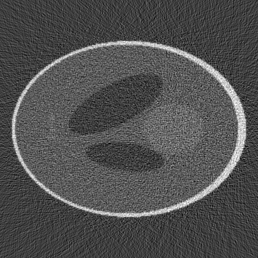
\includegraphics[width=1\textwidth]{sl_fbp_noisy}\\
\vspace{20pt}
$O(N^2 \log N)$
\end{column}
\vrule{}
\begin{column}{0.35\textwidth}
\centering
SIRT\\
\vspace{20pt}

\includegraphics[width=1\textwidth]{sl_art_good}\\
\vspace{20pt}
$O(N^3)$
\end{column}
\vrule{}
\begin{column}{0.35\textwidth}
\centering
FHT-SIRT\\
\vspace{20pt}

\includegraphics[width=1\textwidth]{sl_art_good}\\
\vspace{20pt}
$O(N^2 \log N)$
\end{column}
\end{columns}
\end{frame}

\begin{frame}
\frametitle{Быстрое преобразование Хафа}
\framesubtitle{БПХ, FHT}
\begin{columns}[T,onlytextwidth]
  \hspace*{-0.5cm}
  \begin{column}{0.65\textwidth}
  Приближенный способ вычисления сумм интенсивностей изображения вдоль всевозможных прямых
  \begin{figure}
    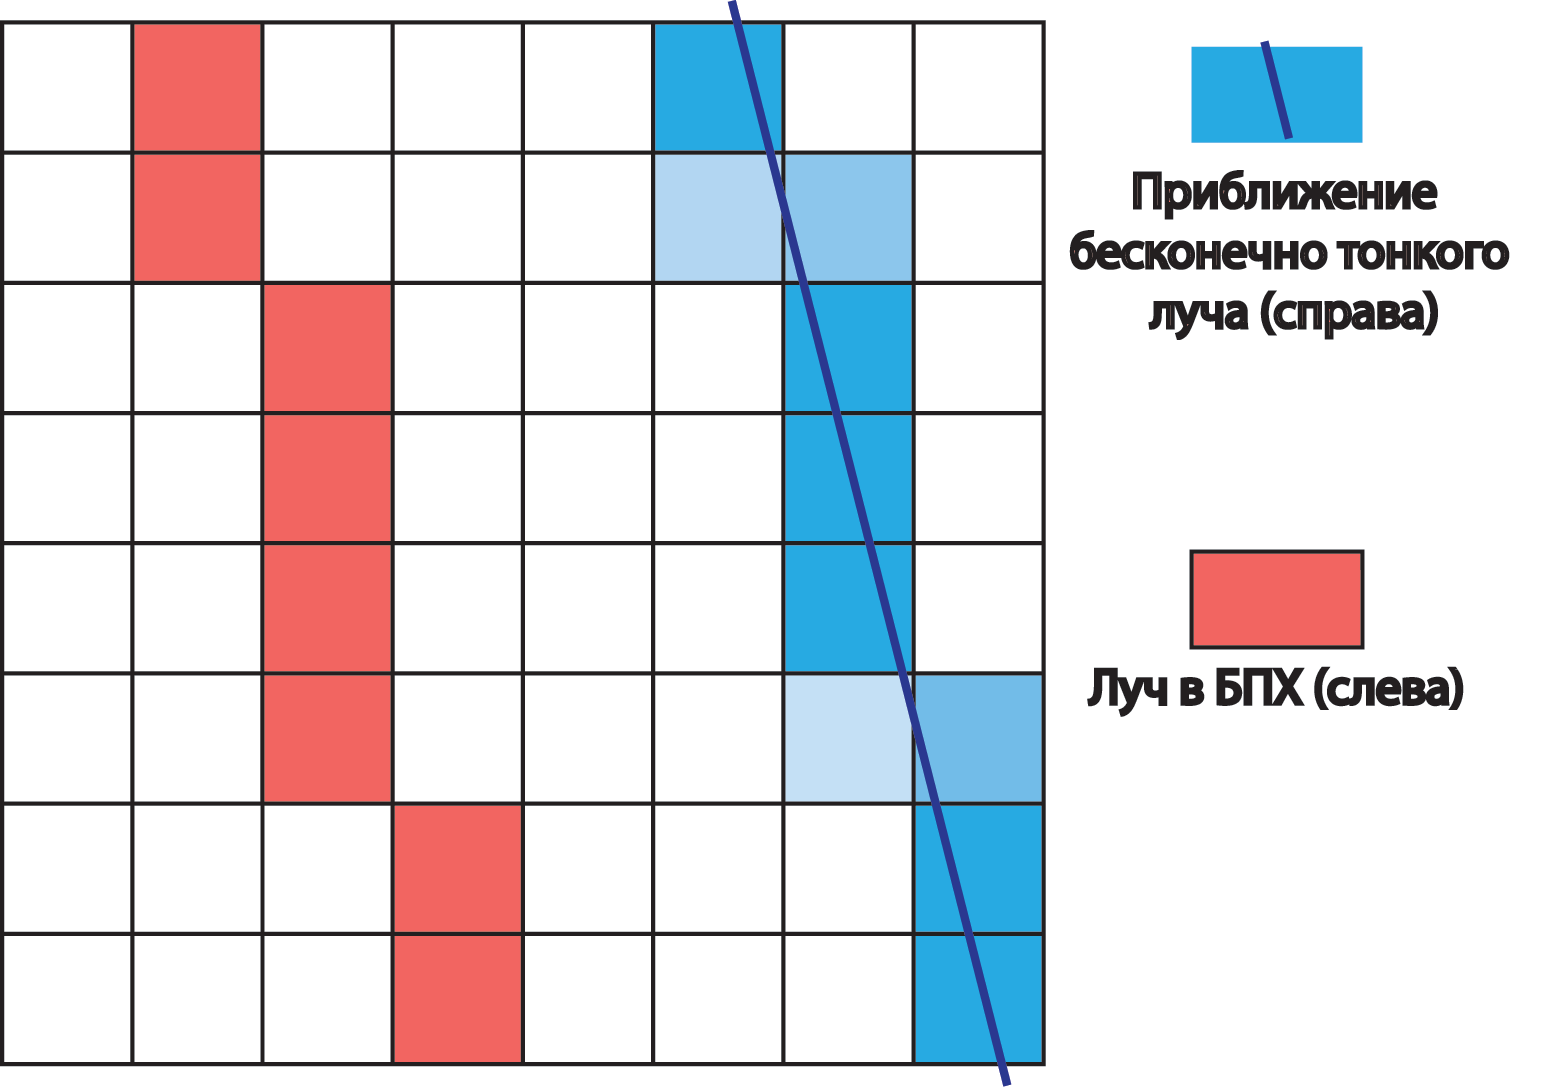
\includegraphics[width=1\textwidth]{fht}
  \end{figure}
  \end{column}
  \begin{column}{0.45\textwidth}
  \begin{itemize}
    \item диадические паттерны суммирования
    \item рекурсивная процедура построения
    \item для больших размеров изображения хорошо приближает прямые (отклонение не превышает  $\frac 1 6 \log N$ ) %\cite{ershov2015dyadic})
    \item асимптотическая сложность $O(N^2 \log N)$
  \end{itemize}
  \end{column}
\end{columns}

\end{frame}

\begin{frame}
\frametitle{Процедура формирования паттернов}
  \begin{figure}
  \centering
    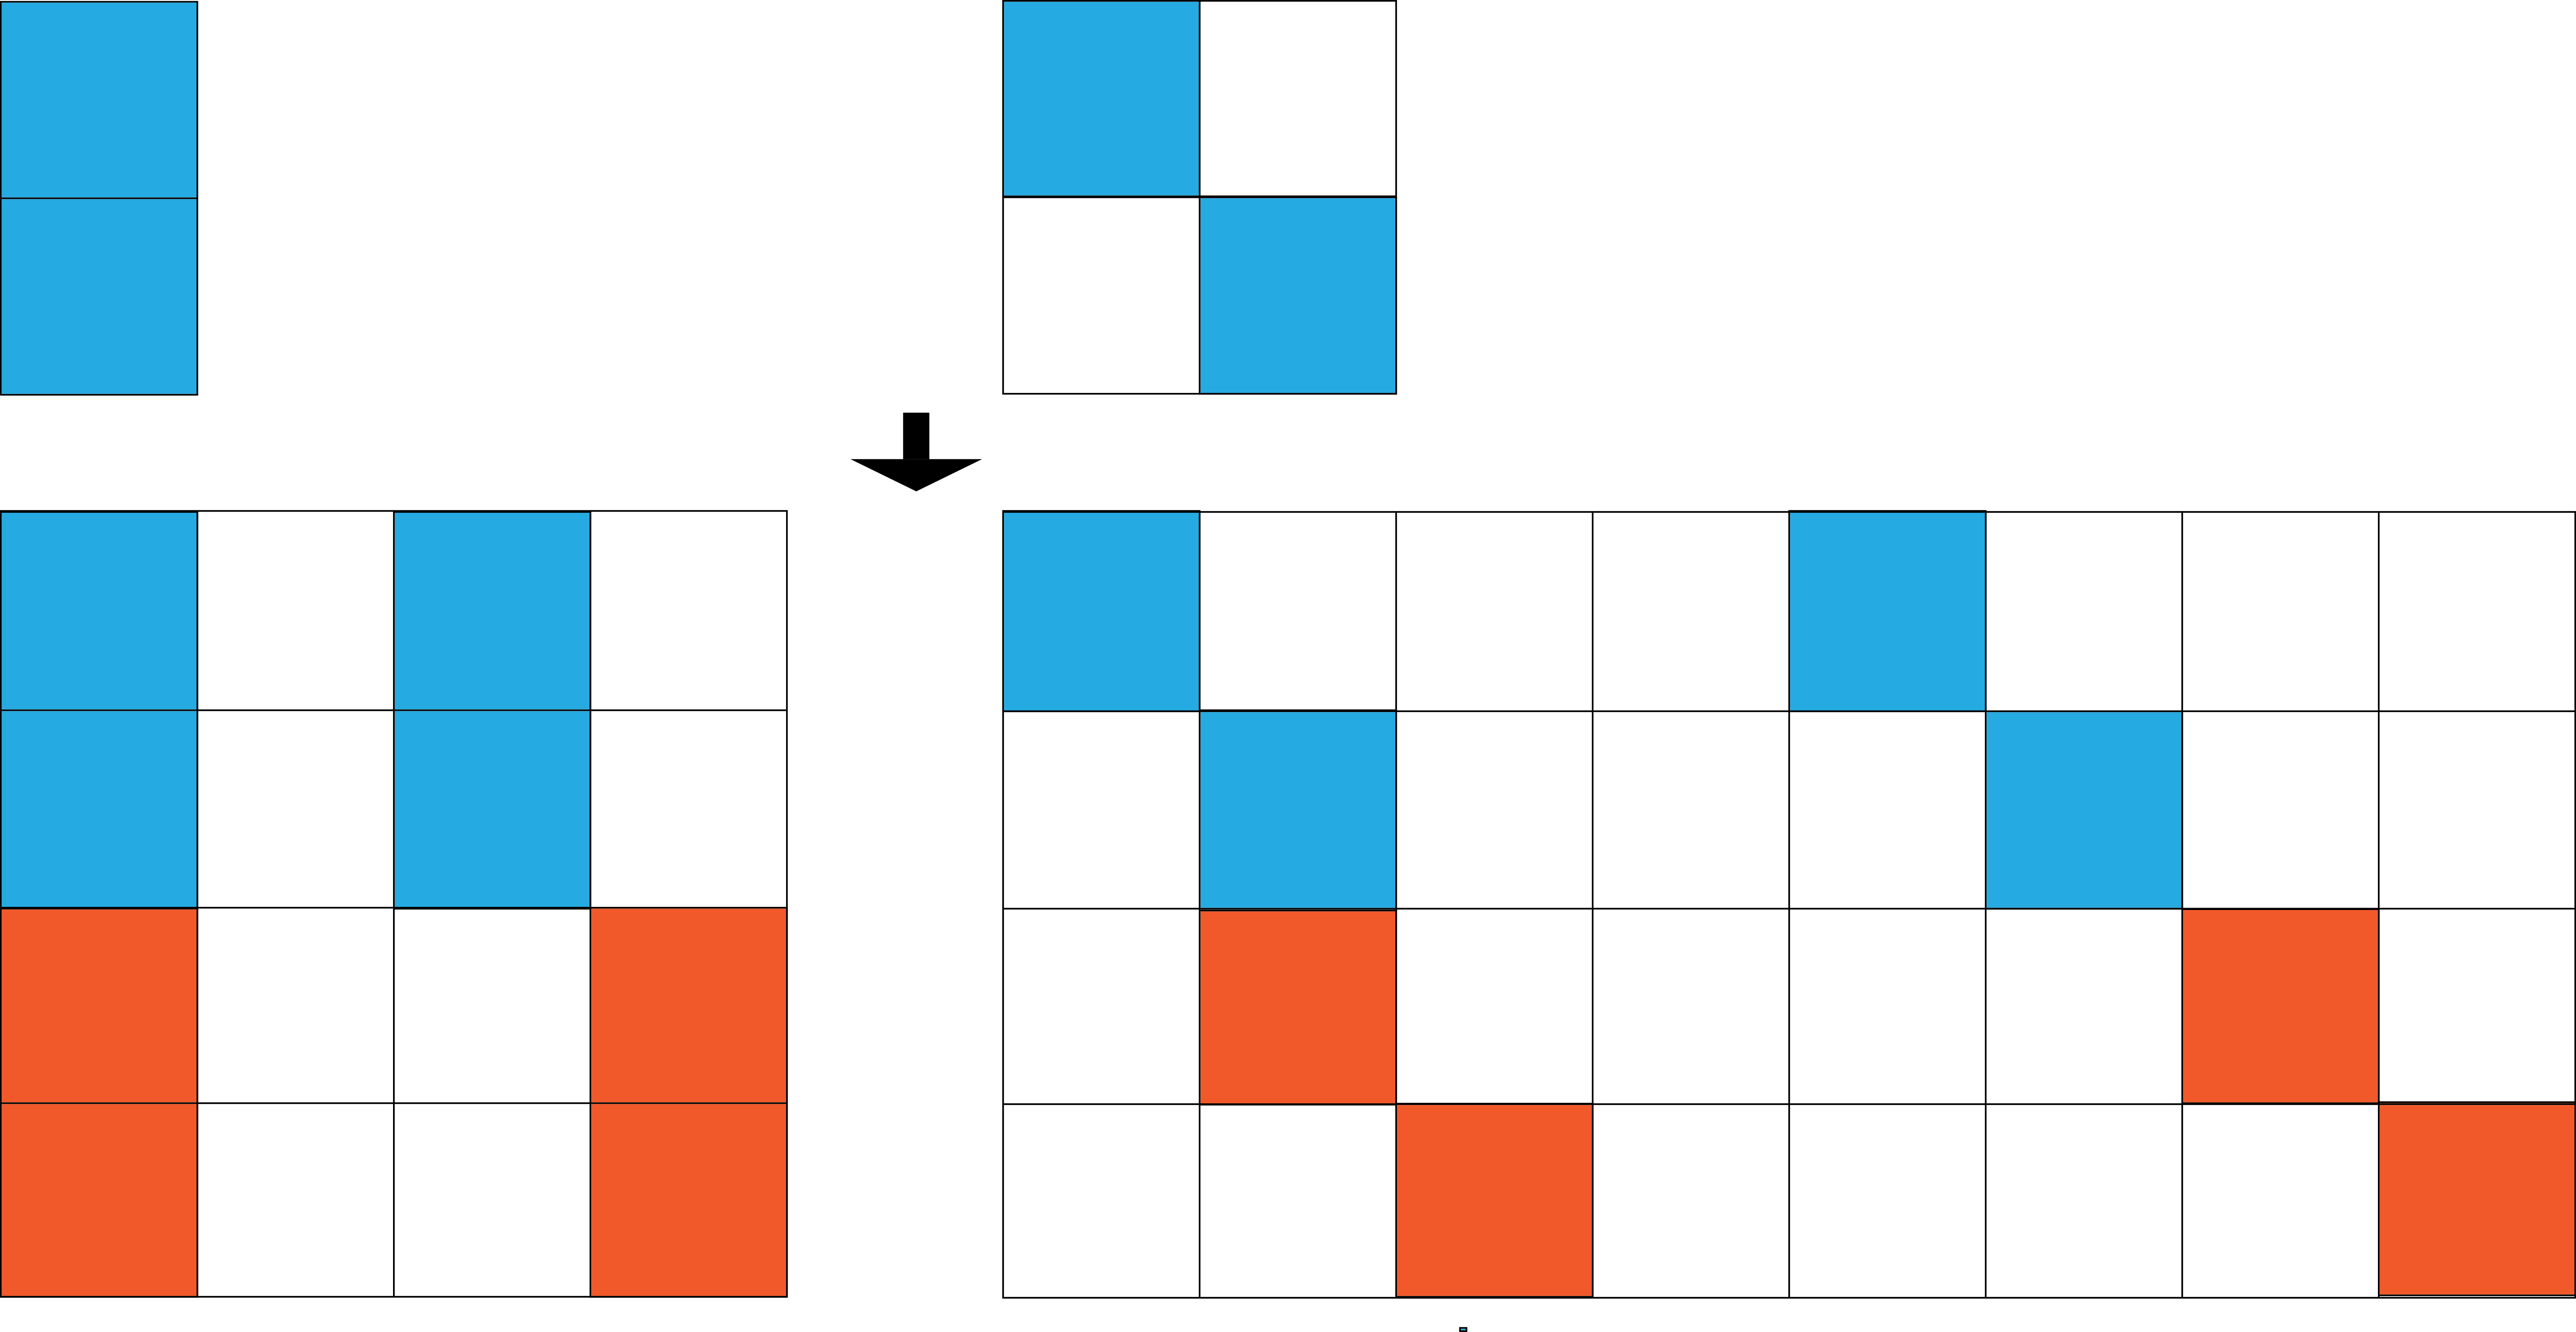
\includegraphics[width=1\textwidth]{../Dissertation/images/part1_img/hough_proc}
  \end{figure}
\end{frame}

\begin{frame}
\frametitle{Быстрое преобразование Хафа}
\framesubtitle{вид матрицы W}
\centering
\begin{columns}

\column{0.2\textwidth}
Обычная проекция \\
$N = 10$ \\
$N_\varphi = 35$

\column{0.3\textwidth}
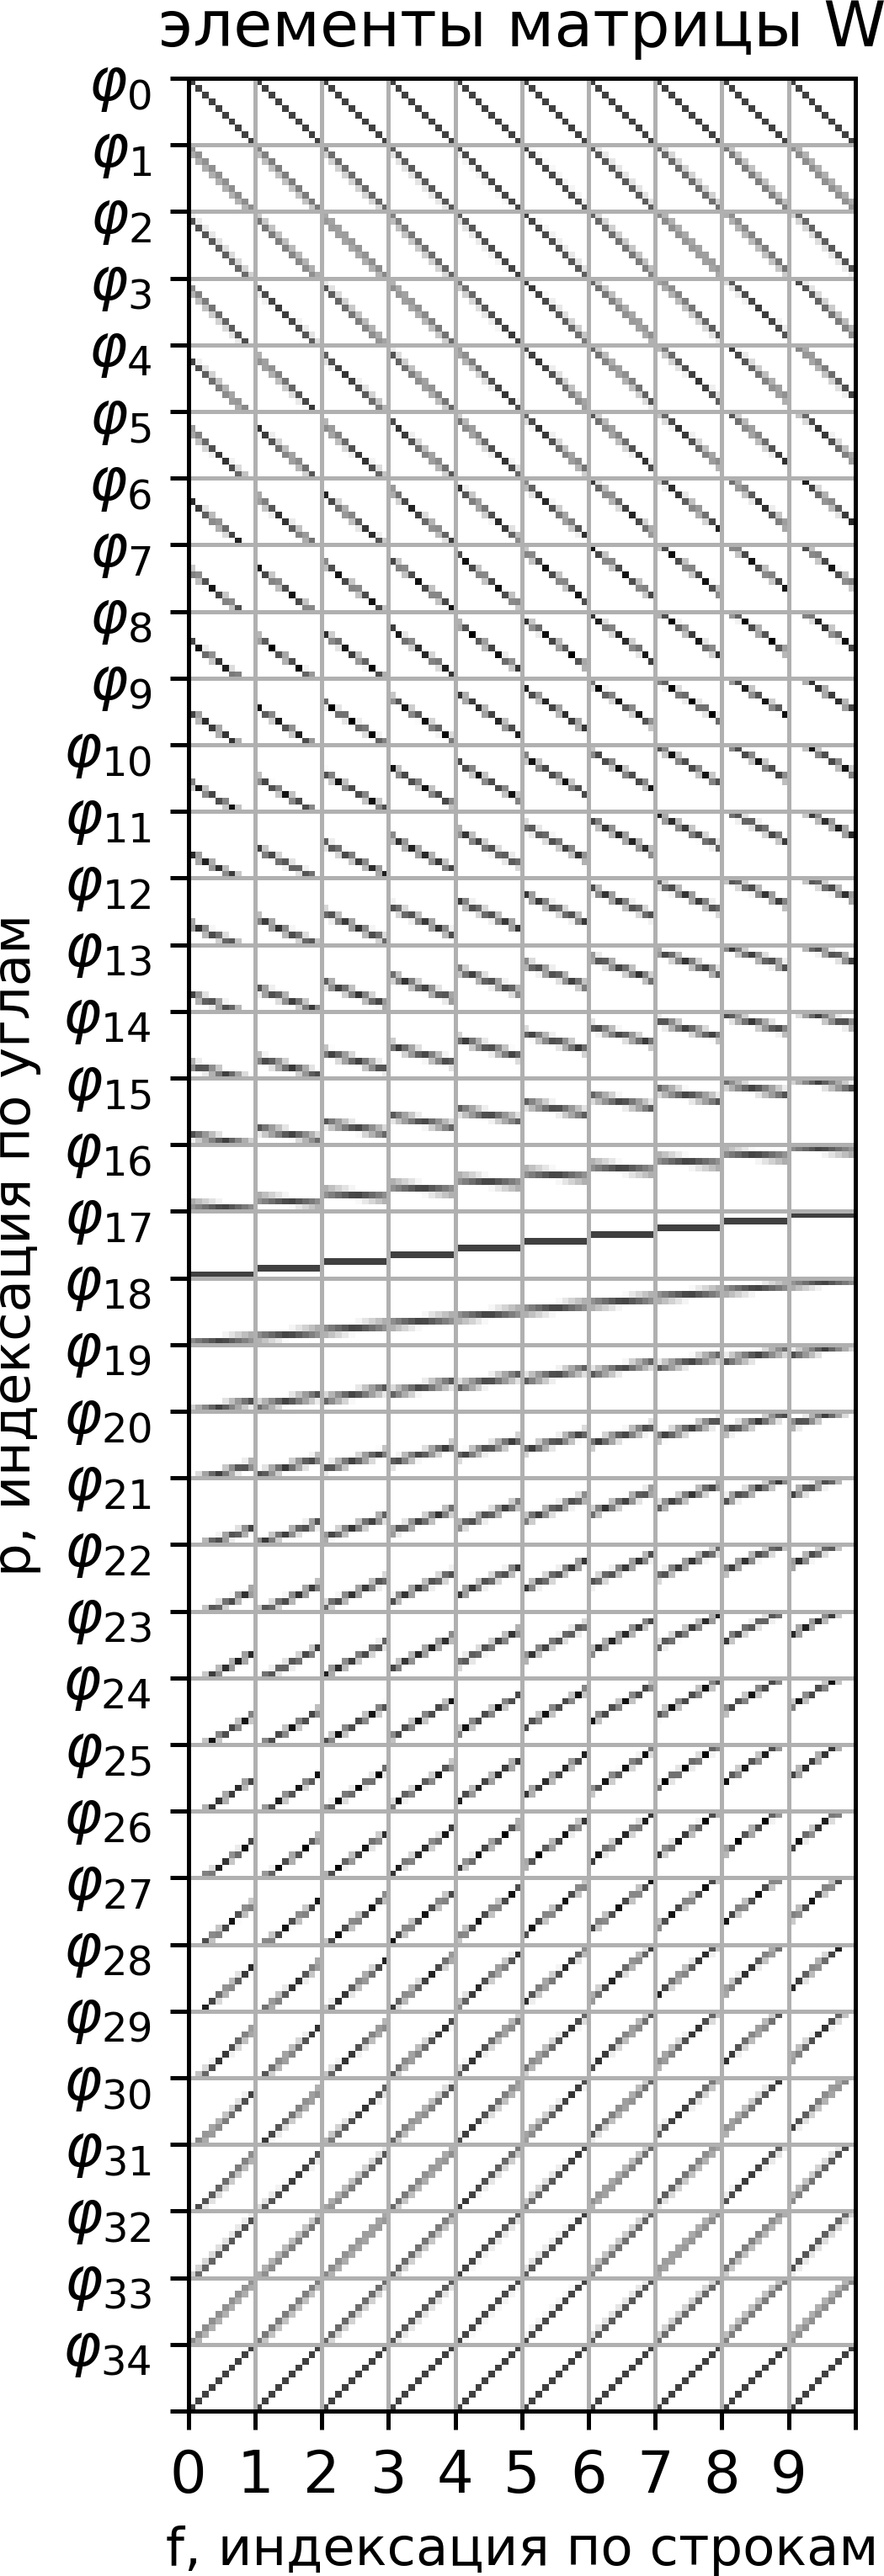
\includegraphics[height=0.7\textheight]{w_matrices/W_10_35_plot.png}

\column{0.3\textwidth}
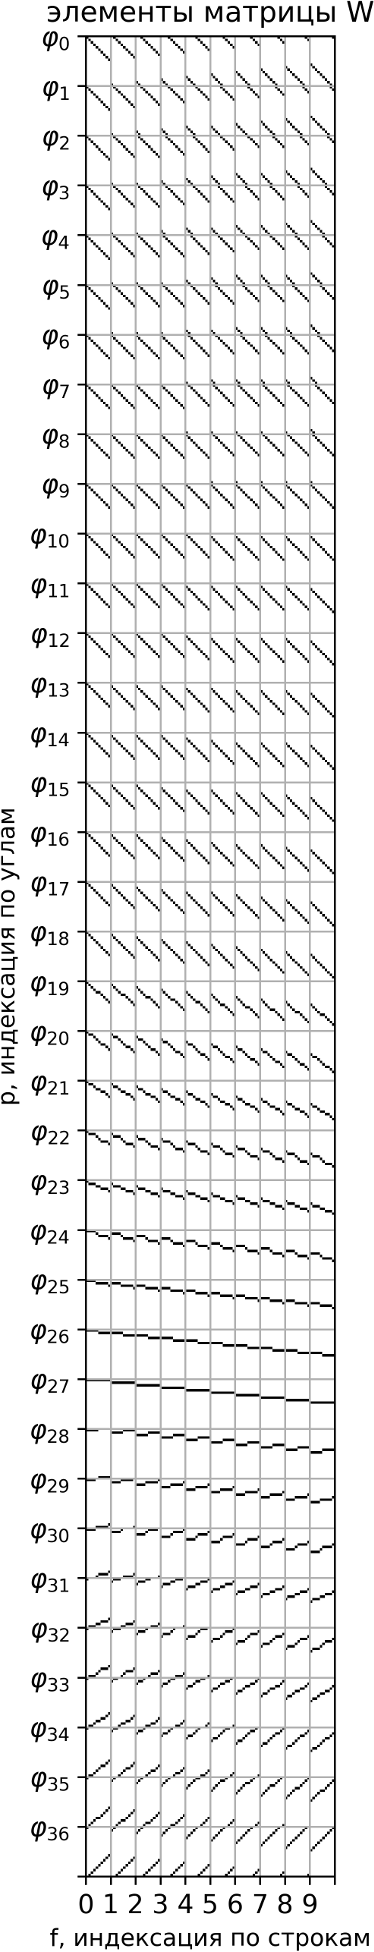
\includegraphics[height=0.80\textheight]{w_matrices/W_FHT_10_plot.png}

\column{0.2\textwidth}
БПХ \\
$N = 10$ \\
$N_\varphi = 37$ \\
\end{columns}
\end{frame}

\begin{frame}
\frametitle{Быстрое преобразование Хафа}
\framesubtitle{вид матрицы W}
\centering
\begin{columns}

\column{0.2\textwidth}
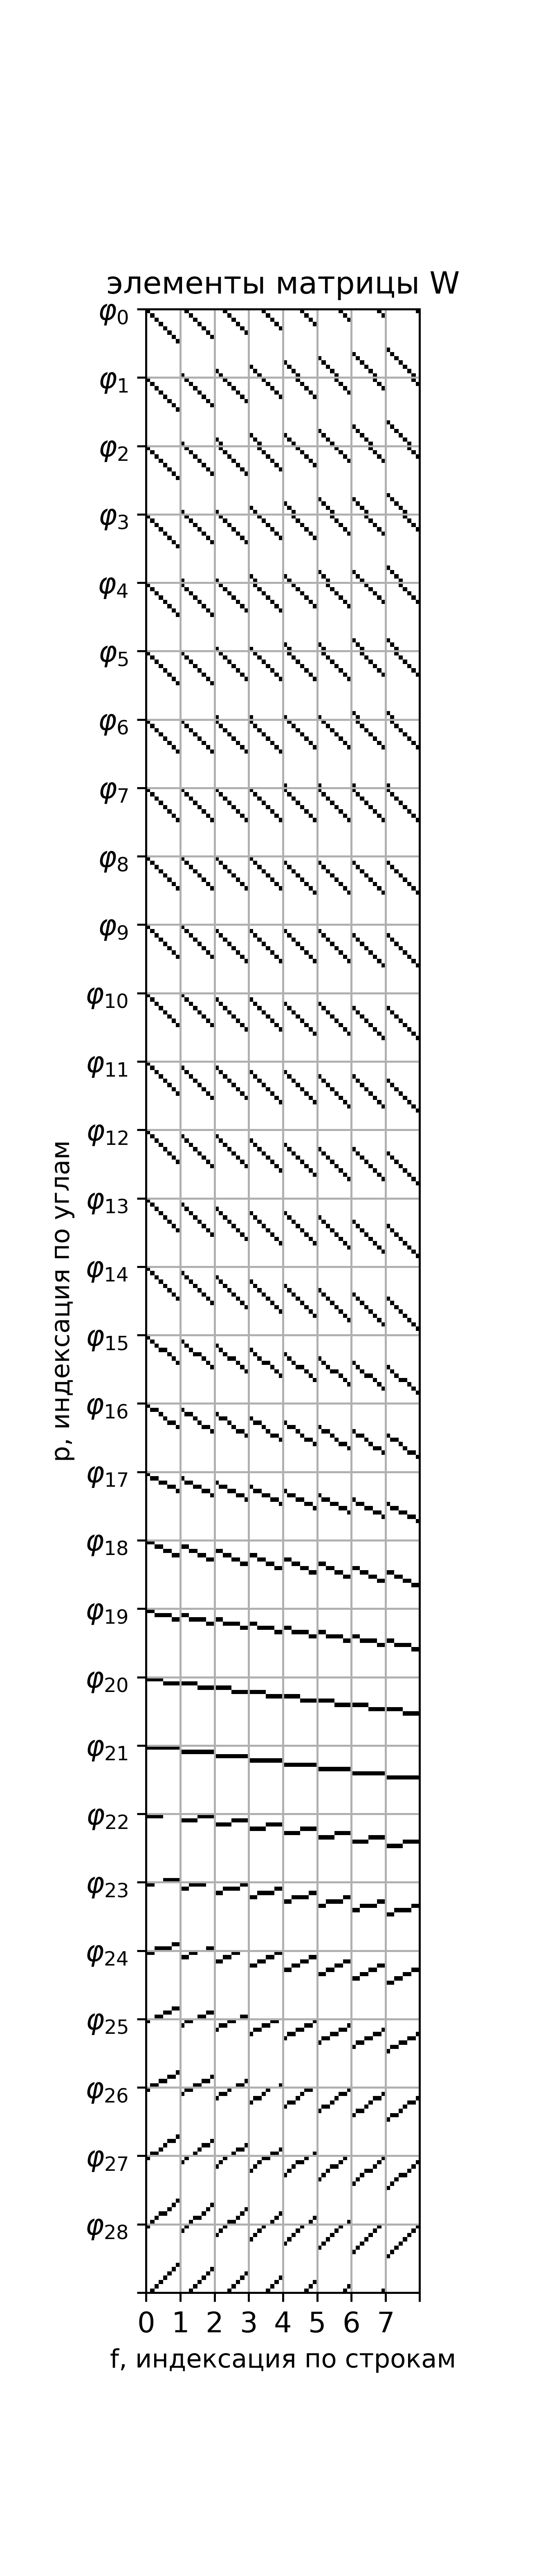
\includegraphics[height=0.9\textheight]{w_matrices/W_FHT_8_plot.png}

\column{0.2\textwidth}
$N = 8$ \\
$N_\varphi = 29$

\column{0.1\textwidth}

\includegraphics[height=0.9\textheight]{w_matrices/W_FHT_16_plot.png}

\column{0.2\textwidth}
$N = 16$ \\
$N_\varphi = 61$


\column{0.1\textwidth}
\includegraphics[height=0.9\textheight]{w_matrices/W_FHT_32_plot.png}

\column{0.2\textwidth}
$N = 32$ \\
$N_\varphi = 125$ \\

\end{columns}

\end{frame}

\begin{frame}
\frametitle{FHT-SIRT}
\framesubtitle{прямая проекция}
\begin{columns}[T,onlytextwidth]
  \hspace*{-0.5cm}
  \begin{column}{0.65\textwidth}
  \begin{figure}
    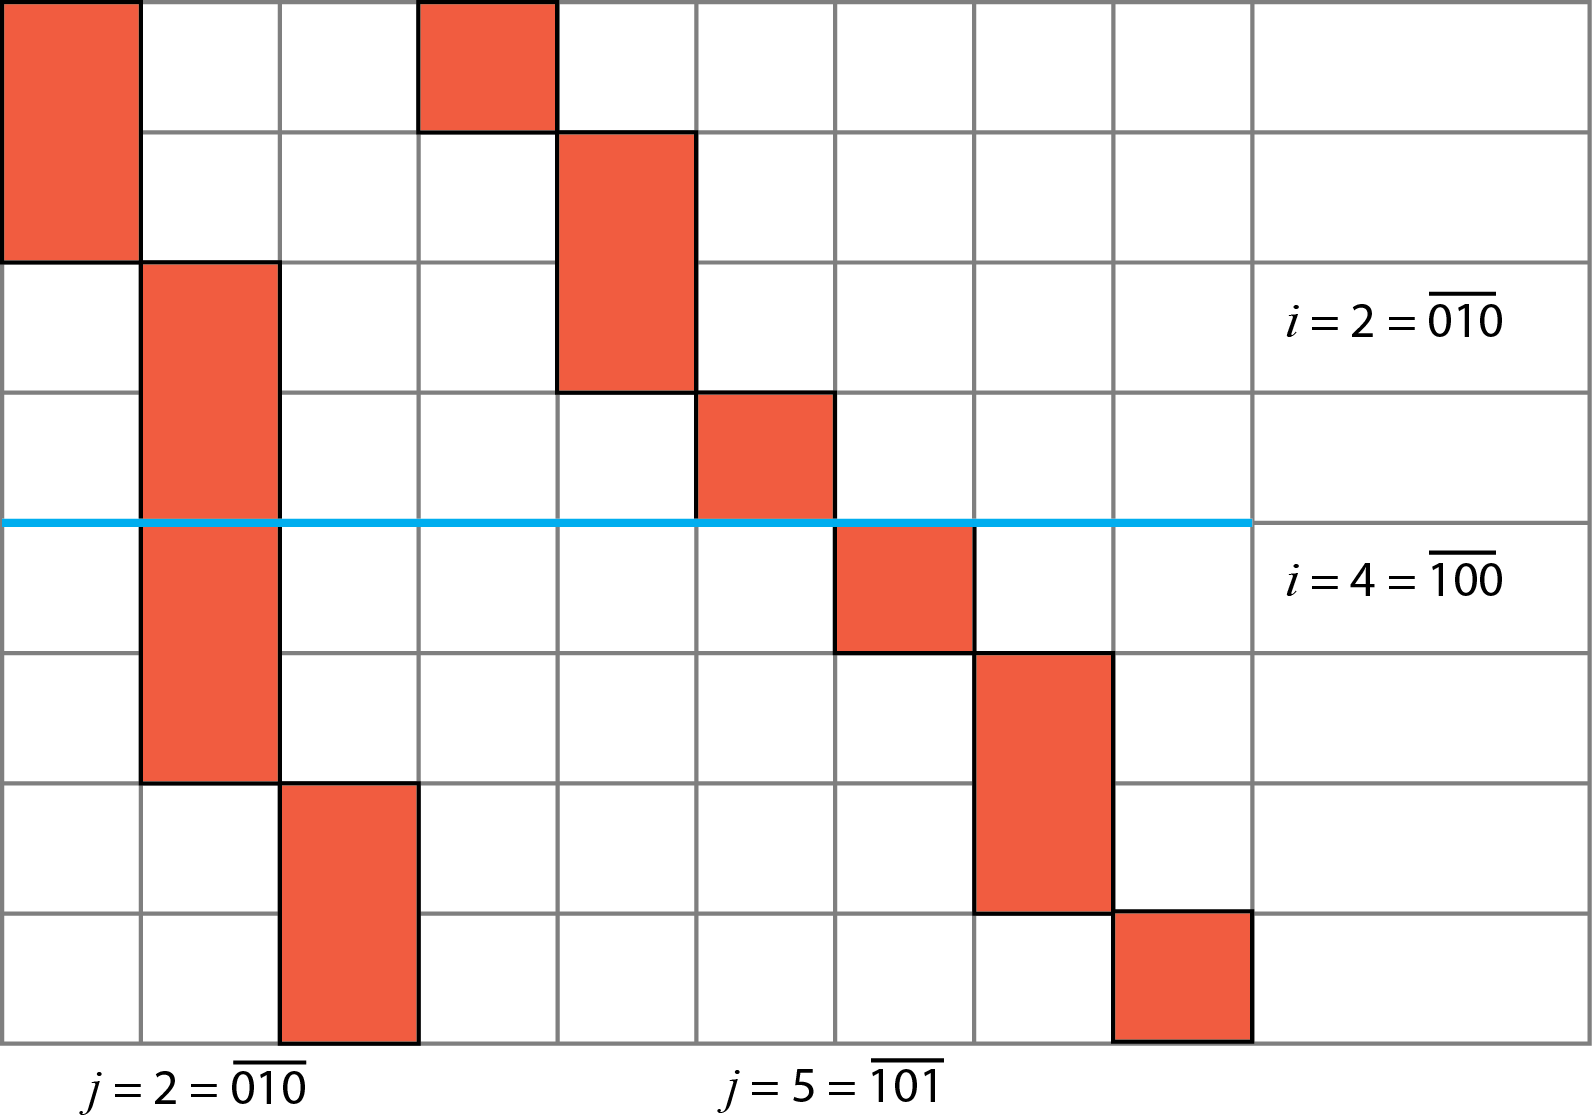
\includegraphics[width=\textwidth]{../Dissertation/images/part1_img/pattern_structure}
  \end{figure}
  \end{column}
  \begin{column}{0.45\textwidth}
    Углы в БПХ делятся на 4 группы:
    \begin{equation} \notag
    \begin{array}{lll}
    \alpha^\rom{1}_i &= \pi - & \arctan{\frac{N-1-i}{N-1}} \\
    \alpha^\rom{2}_i &= &\arctan{\frac{i - (N-1)}{N-1}} \\
    \alpha^\rom{3}_i &= \frac \pi 2 - & \arctan{\frac{3(N-1)-i}{N-1}} \\
    \alpha^\rom{4}_i &= \frac \pi 2 - & \arctan{\frac{i - 3(N-1)}{N-1}}
    \end{array}
    \end{equation}

    Вычисление прямой проекции в шаге FHT-SIRT имеет вид 
        $\mathrm W = \left( \mathrm  W^\rom{1}\ \mathrm W^\rom{2}\ \mathrm  W^\rom{3}\ \mathrm  W^\rom{4} \right)^{\mathrm T}$.
  \end{column}
\end{columns}
\end{frame}


\begin{frame}
\frametitle{FHT-SIRT}
\framesubtitle{обратная проекция}

\begingroup
\small
\vspace{-0.5cm}
\newtheorem{myth}{Лемма}\
\begin{myth}
Пусть $pattern_j$ --- вертикальный паттерн скоса для j'ой строки преобразования Хафа изображения высотой $M_s = 2^n$.
Тогда имеет место равенство:
\begin{equation} \notag
\label{statement1}
\begin{array}{l l}
pattern_j[i] = pattern_i[j] & \quad  i,j \in \overline{1, 2^n},
\end{array}
\end{equation}
т. е. матрица, составленная из паттернов скоса, записанных в качестве столбцов, симметрична.
\end{myth}
\endgroup
\noindent\rule{8cm}{0.4pt}
\vspace{0.3cm}

Откуда следует, что ${W^{\mathrm K}} ^ {\mathrm T} = W^{\mathrm K}$, а значит
$$
W^{\mathrm T} q = \sum_{K=\rom{1}}^{K=\rom{4}}{W^{\mathrm K} q}
$$

\end{frame}


\begin{frame}
\frametitle{FHT-SIRT}
\framesubtitle{исследование работы}

\begin{columns}[T,onlytextwidth]
  \hspace*{-0.5cm}
  \begin{column}{0.53\textwidth}
    \begin{figure}
      \centering
      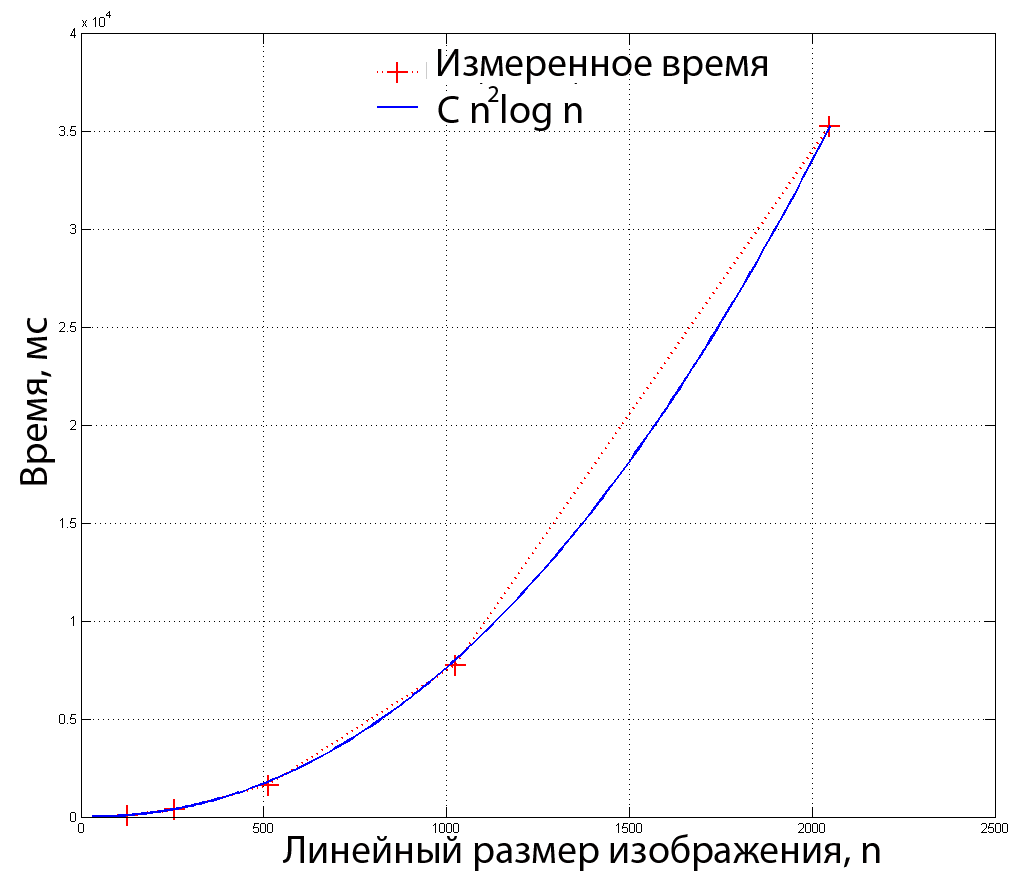
\includegraphics[width=\textwidth]{fht_sirt_time_30_it}
      \caption{Время работы 30 итераций алгоритма}
    \end{figure}
  \end{column}
  \begin{column}{0.6\textwidth}
    \begin{figure}
      \centering
      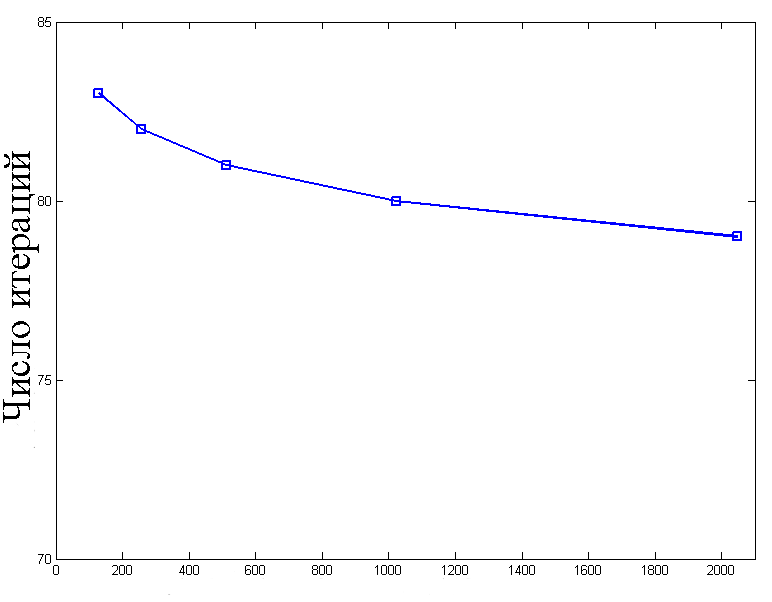
\includegraphics[width=\textwidth]{../Dissertation/images/part1_img/it_till_stop}
      \caption{количество итераций до заданного уровня ошибки на разных размерах изображения}
    \end{figure}
  \end{column}
\end{columns}
\end{frame}


% ======================================================
% ================= Сравнение с SART ===================
% ======================================================
\begin{frame}
\frametitle{FHT-SIRT}
\framesubtitle{сравнение с SART}
  \begin{figure}
  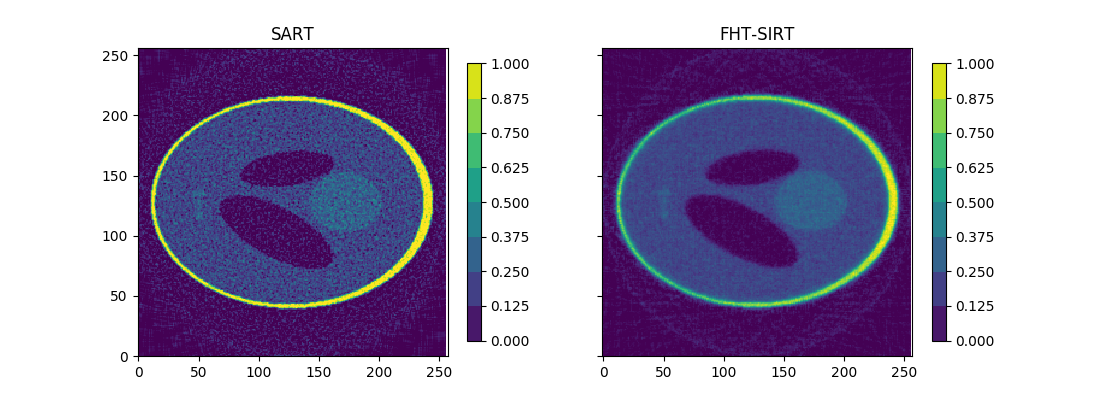
\includegraphics[width=0.8\textwidth]{sart__fht_sirt}
  \end{figure}

% \hline
\vspace{0.5cm}


\small
\begin{tabular}{c|c c}
    метод & SART & FHT-SIRT \\ \vspace{5pt}
    количество итераций & 1 & 40 \\ \vspace{5pt}
    время & 0.931c & 0.935c \\ \vspace{5pt}
    ошибка & 11.8845 & 16.1192 \\ \vspace{5pt}
    СКО & 0.3278 & 0.3882 \\ \vspace{5pt}
    N & 256 & 256 \\
\end{tabular}

\end{frame}


\begin{frame}
\frametitle{FHT-SIRT}
\framesubtitle{сравнение с SART: кросс-секции}
\begin{columns}[T,onlytextwidth]
  \hspace*{-1cm}
  \begin{column}{0.4\textwidth}
    \begin{figure}
      \centering
      %\vspace{0.75cm}
      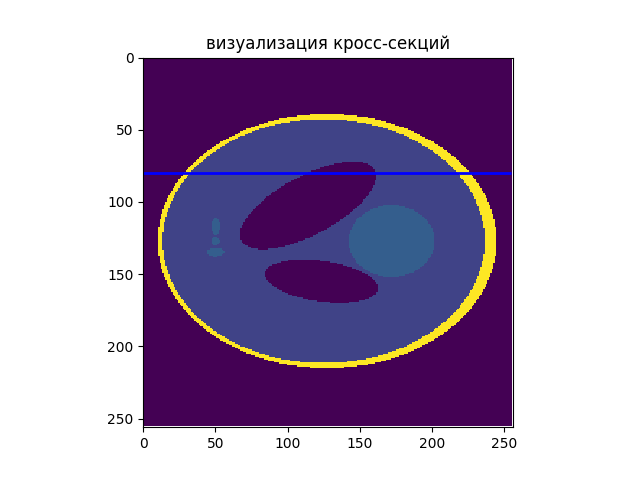
\includegraphics[width=1.5\textwidth]{cs_80_viz}
    \end{figure}
  \end{column}
  \begin{column}{0.6\textwidth}
    \begin{figure}
      \centering
      %\vspace{-1cm}
      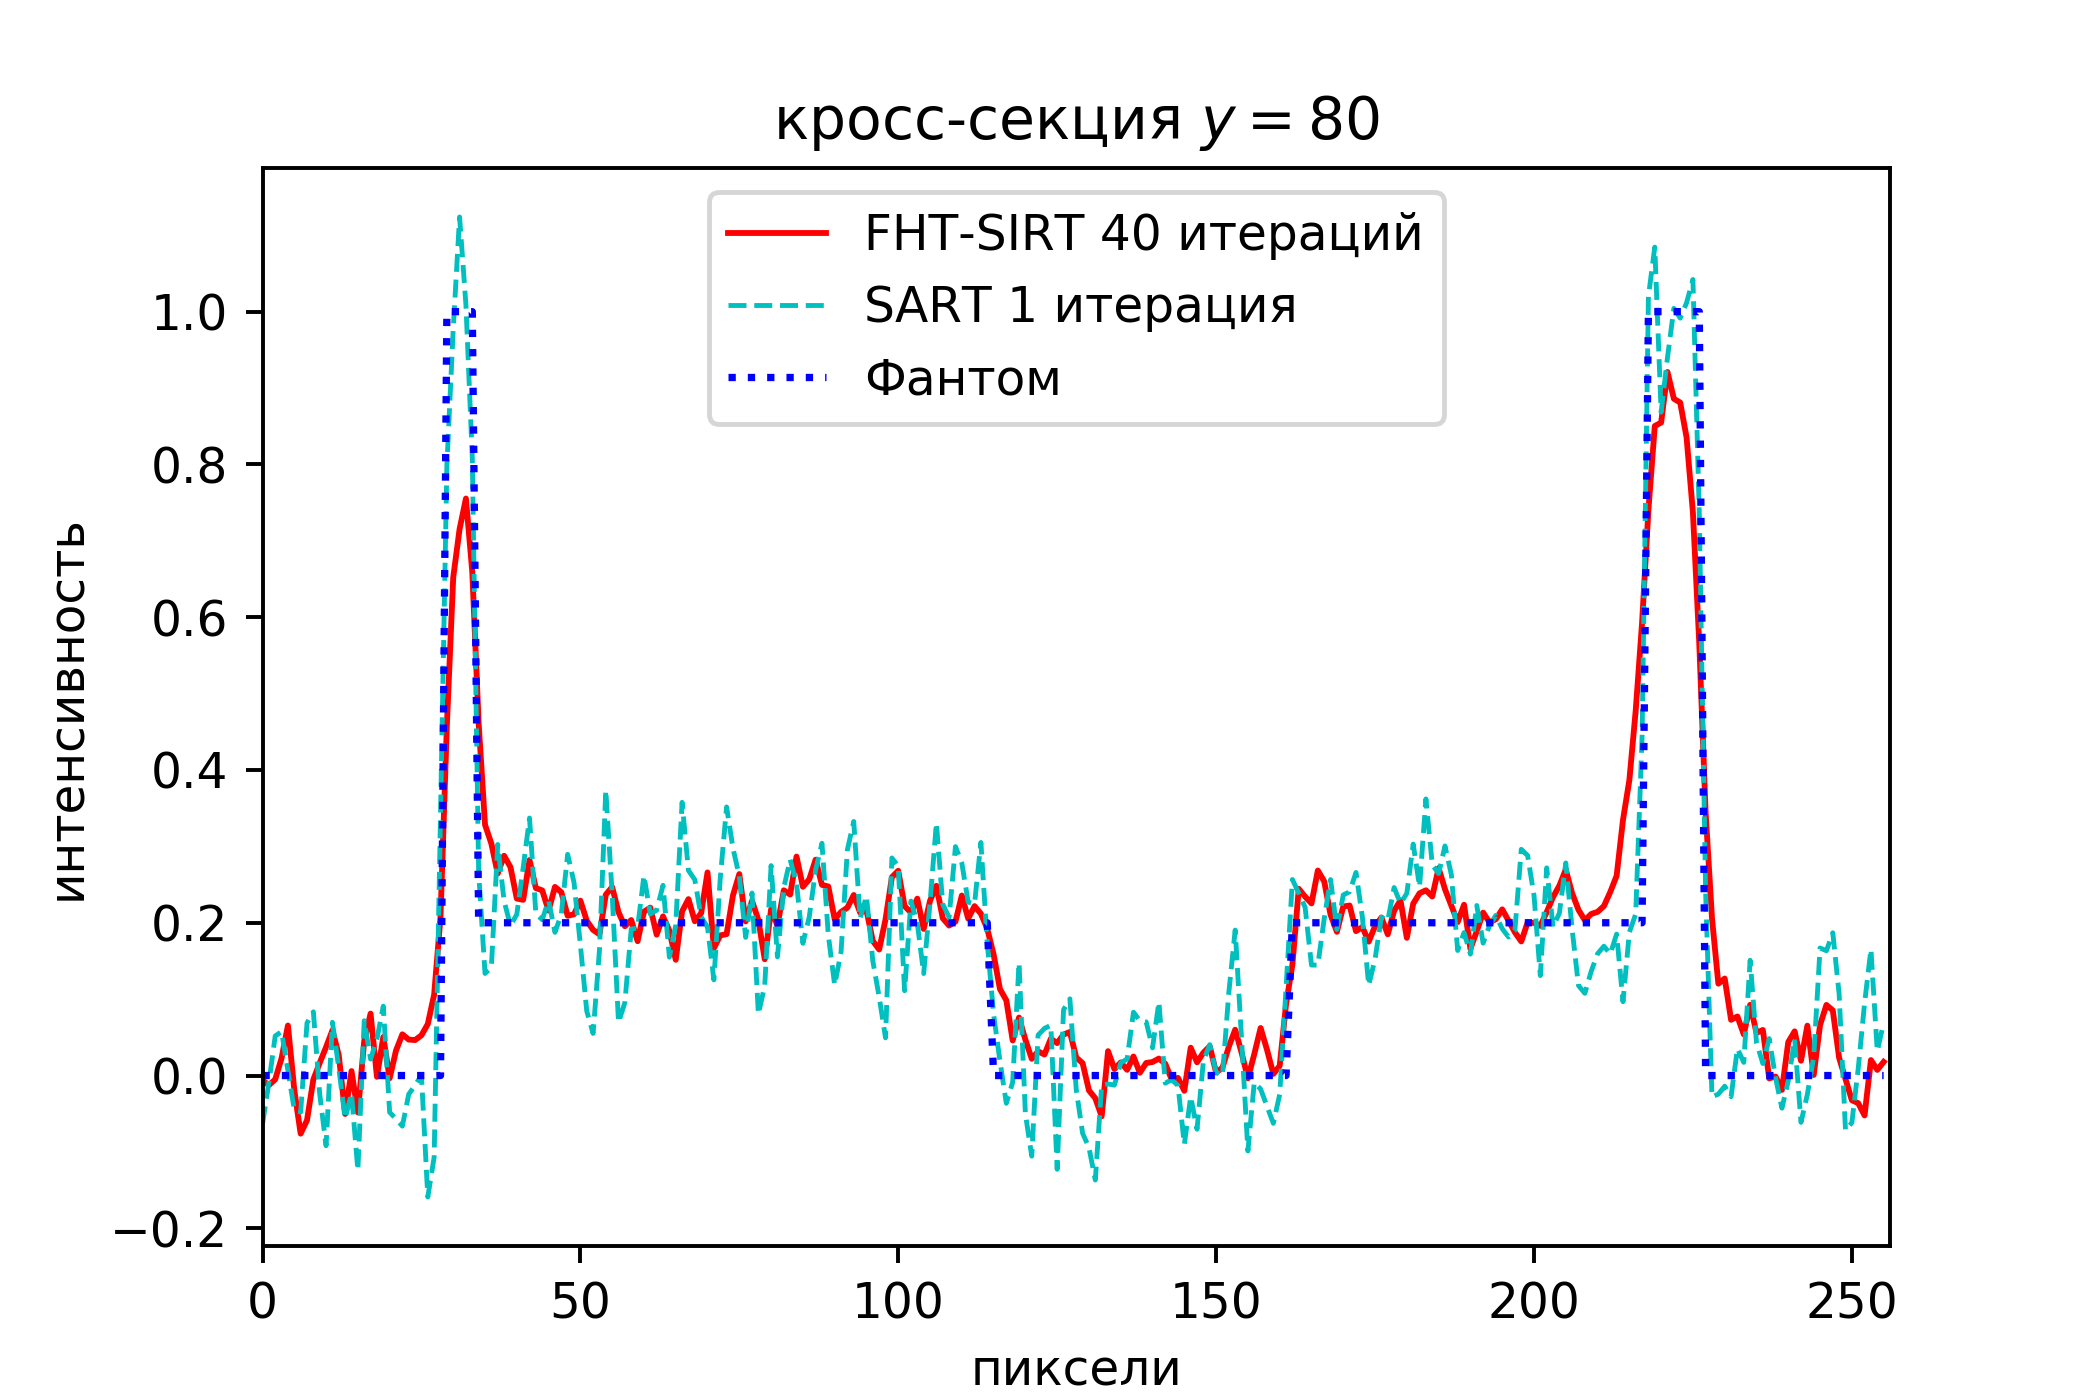
\includegraphics[width=1.2\textwidth]{cs_80}
    \end{figure}
  \end{column}
\end{columns}
\end{frame}

\begin{frame}
\frametitle{FHT-SIRT}
\framesubtitle{сравнение с SART: кросс-секции}
\begin{columns}[T,onlytextwidth]
  \hspace*{-1cm}
  \begin{column}{0.4\textwidth}
    \begin{figure}
      \centering
      %\vspace{0.75cm}
      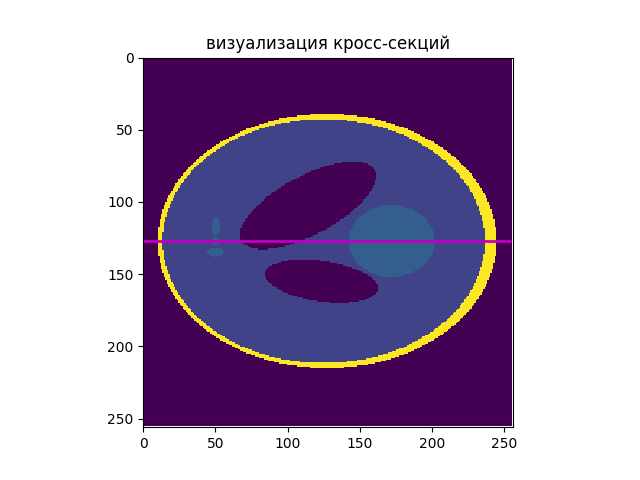
\includegraphics[width=1.5\textwidth]{cs_127_viz}
    \end{figure}
  \end{column}
  \begin{column}{0.6\textwidth}
    \begin{figure}
      \centering
      %\vspace{1cm}
      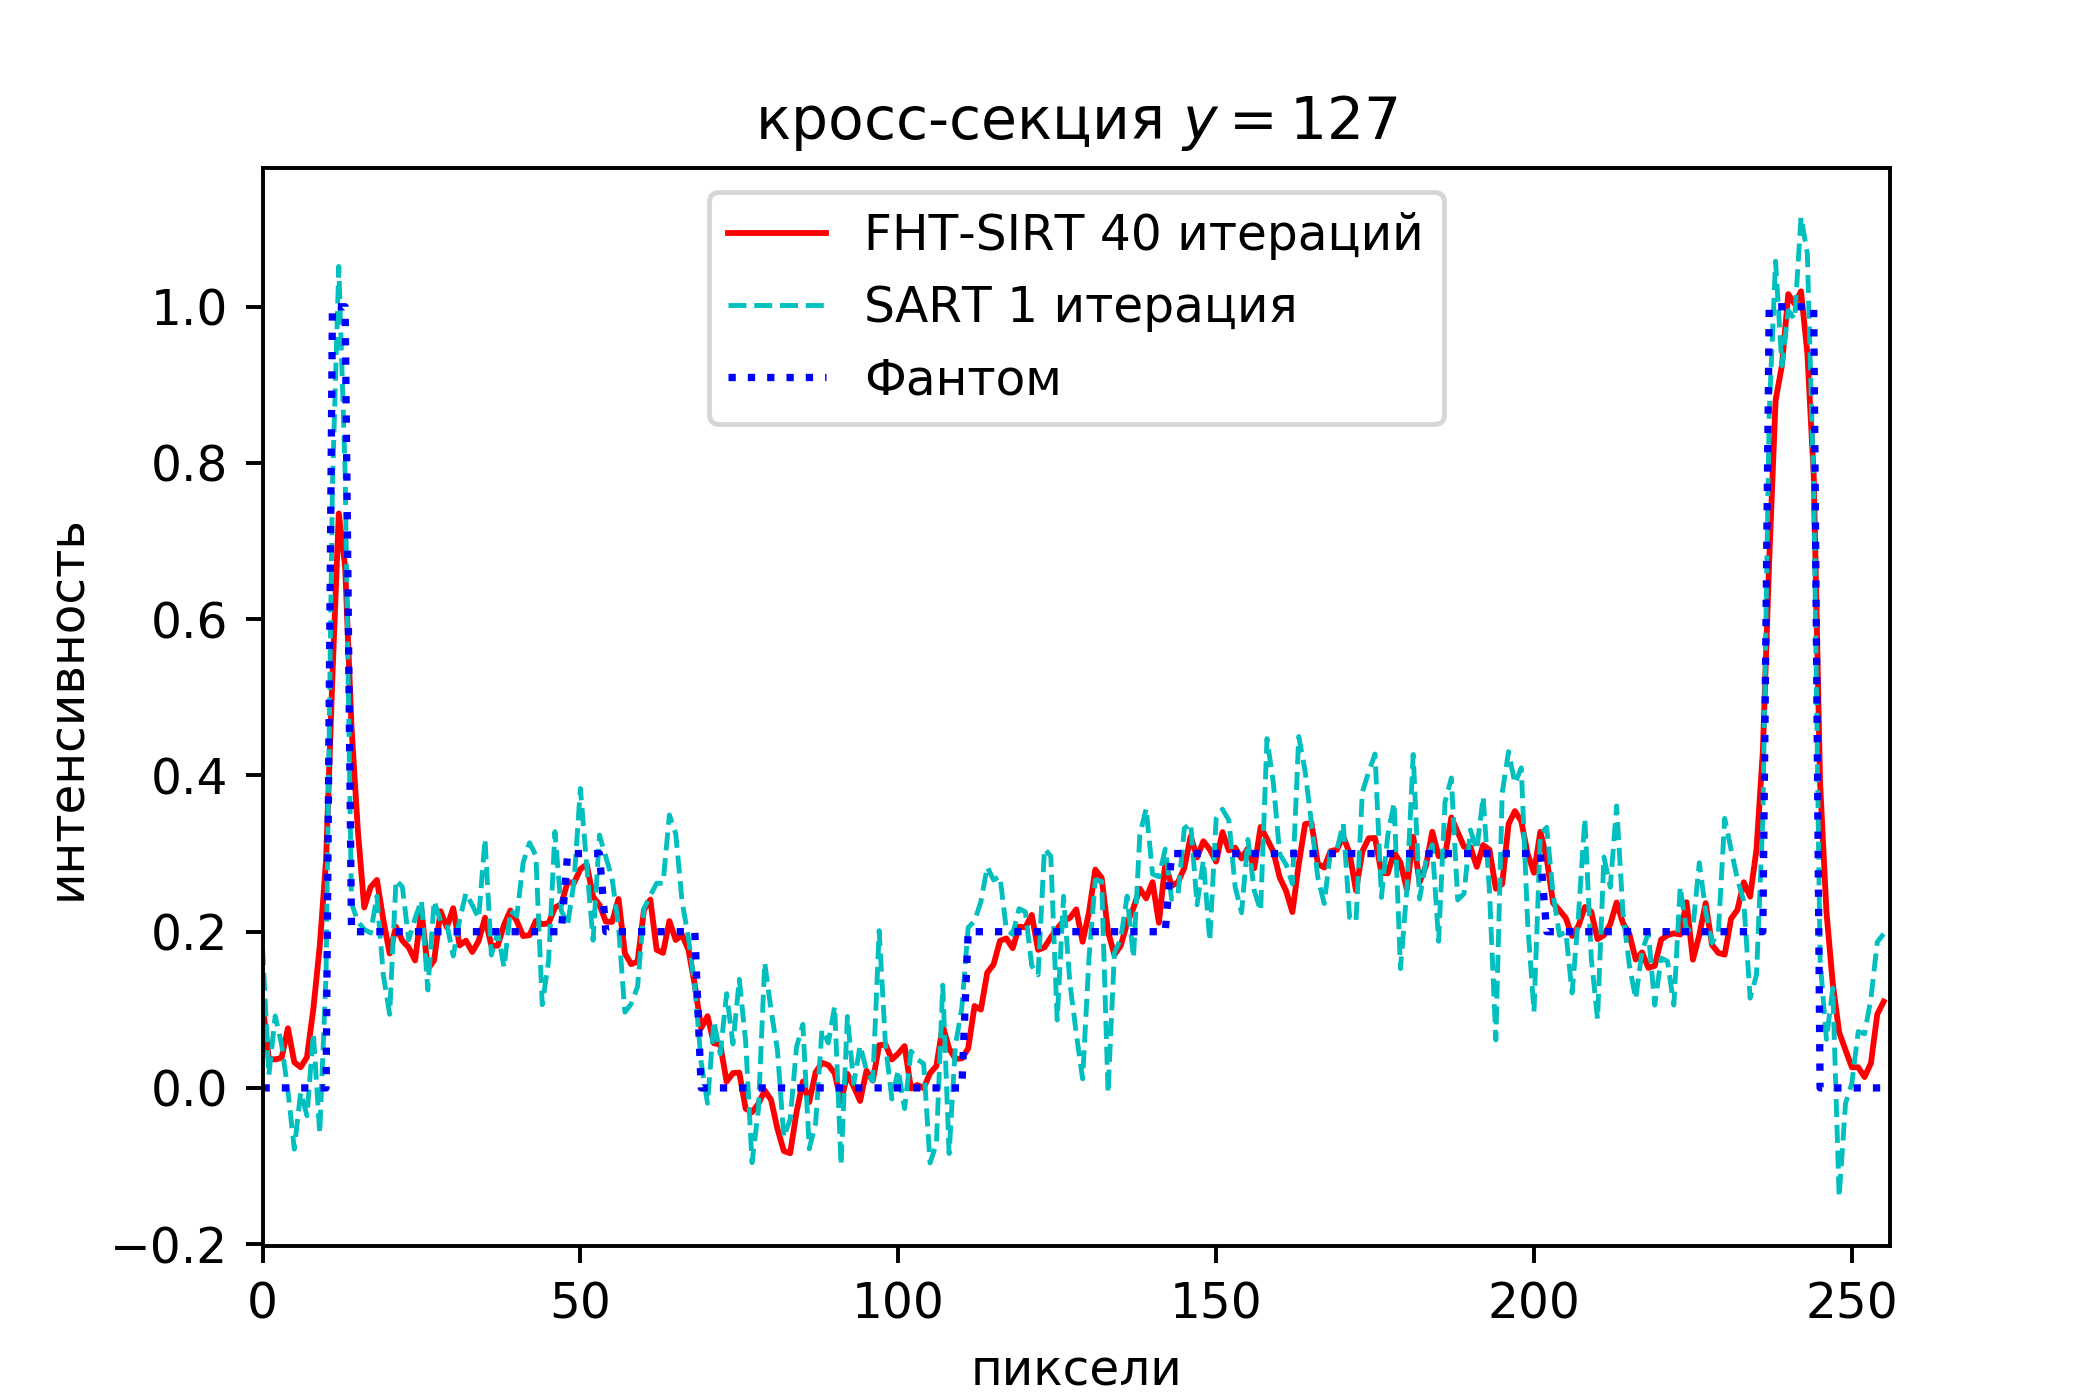
\includegraphics[width=1.2\textwidth]{cs_127}
    \end{figure}
  \end{column}
\end{columns}
\end{frame}


\begin{frame}
\frametitle{FHT-SIRT}
\framesubtitle{сравнение с SART: кросс-секции}
\begin{columns}[T,onlytextwidth]
  \hspace*{-1cm}
  \begin{column}{0.4\textwidth}
    \begin{figure}
      \centering
      %\vspace{0.75cm}
      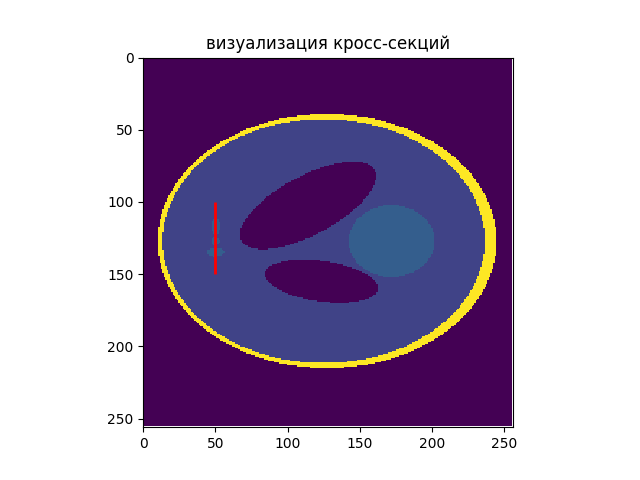
\includegraphics[width=1.5\textwidth]{cs_v_50_viz}
    \end{figure}
  \end{column}
  \begin{column}{0.6\textwidth}
    \begin{figure}
      \centering
      %\vspace{-1cm}
      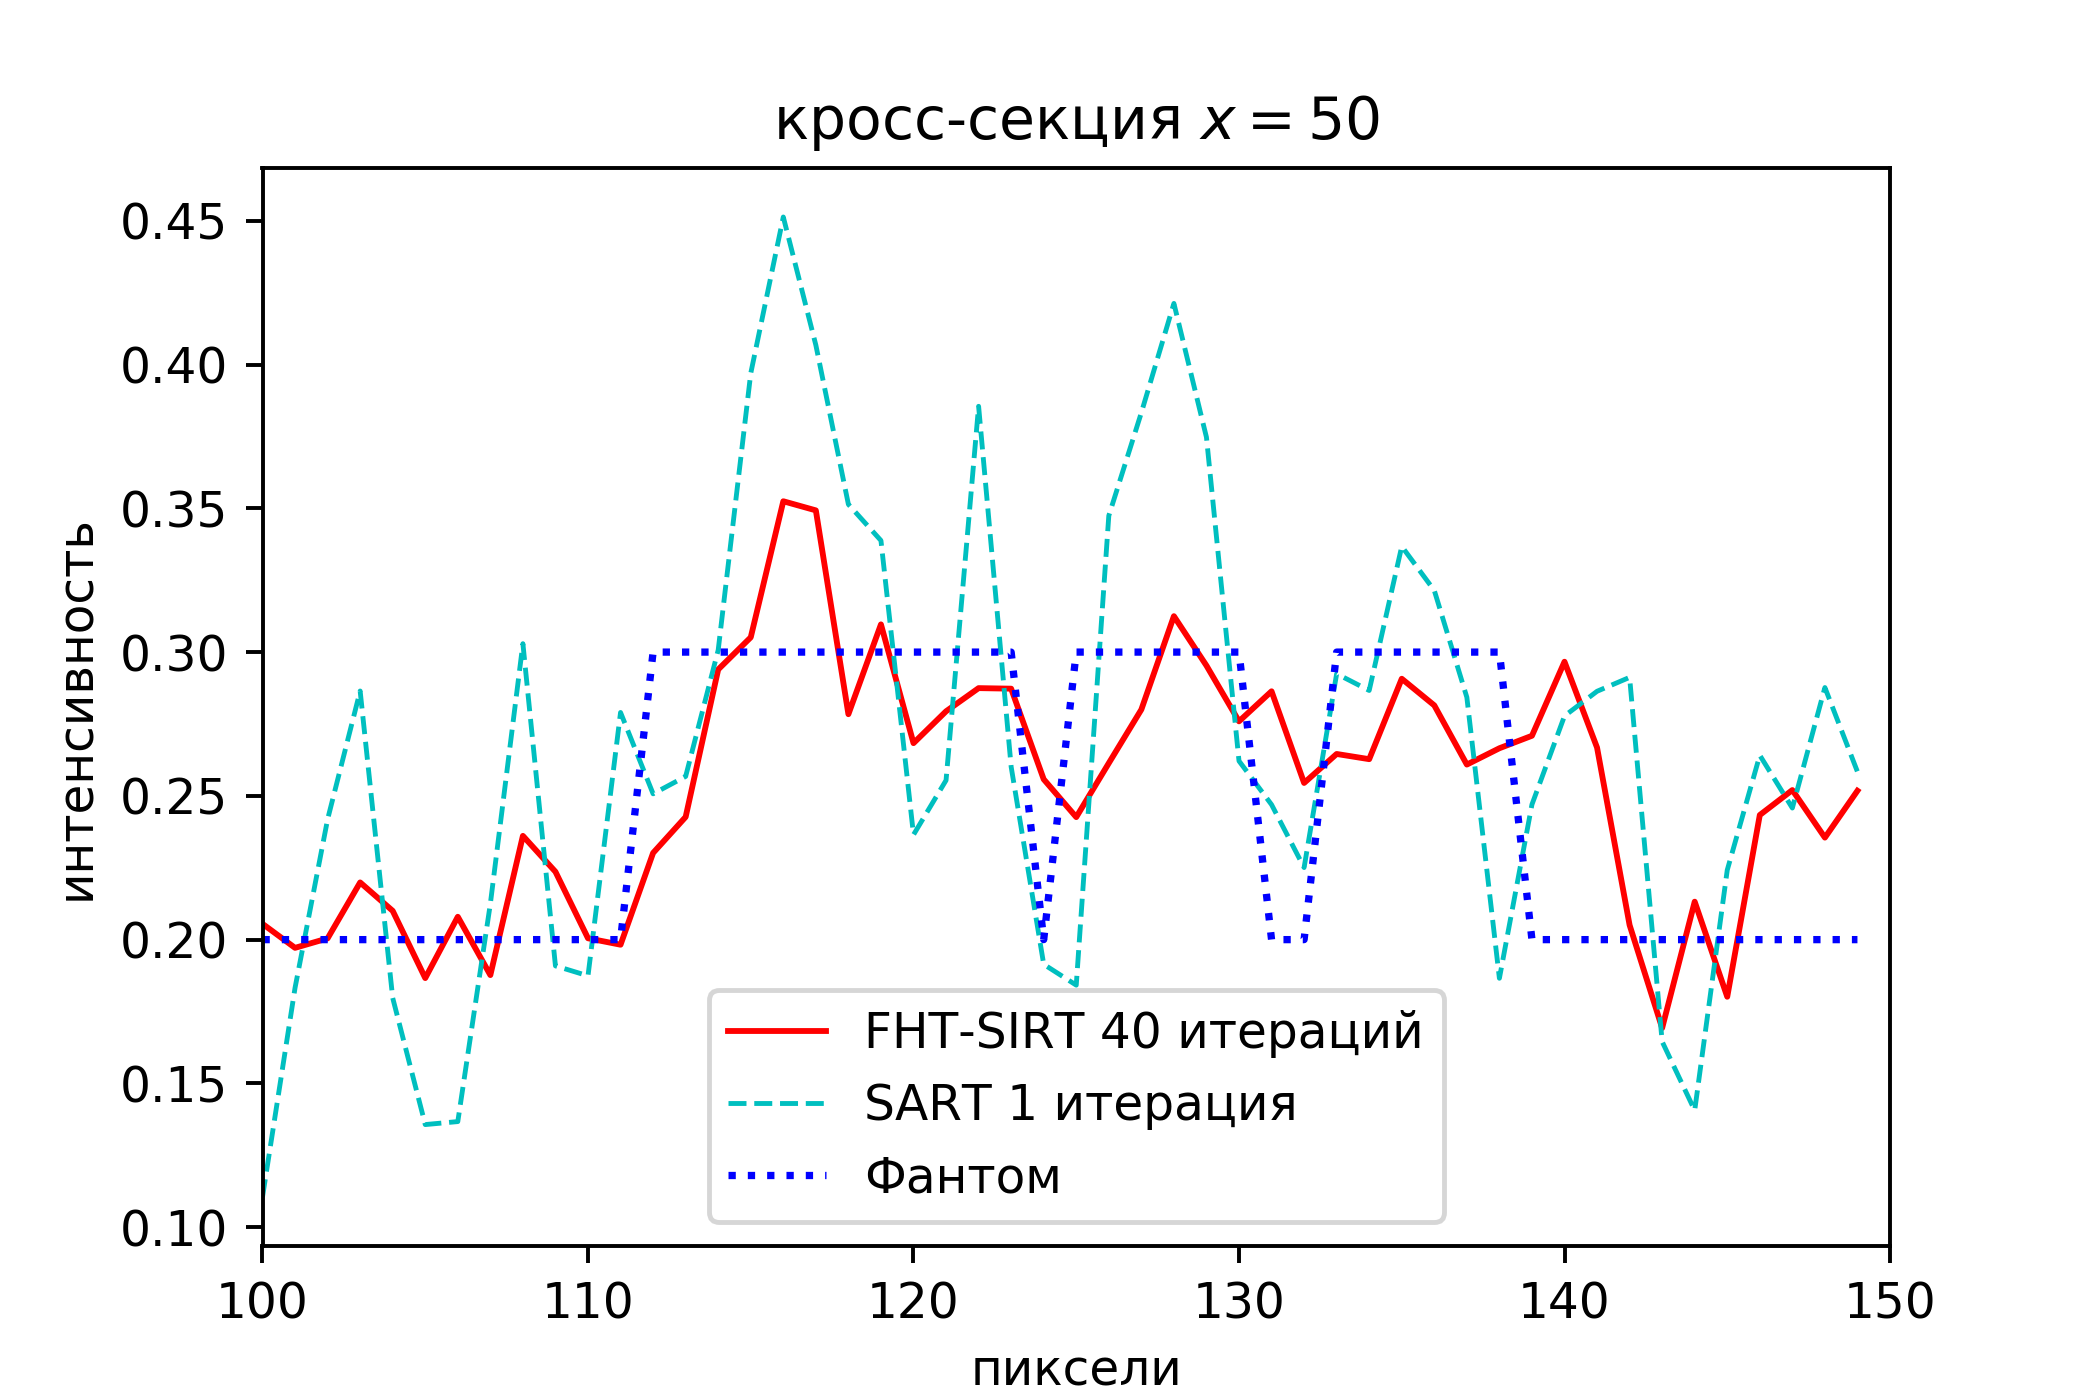
\includegraphics[width=1.2\textwidth]{cs_v_50}
    \end{figure}
  \end{column}
\end{columns}
\end{frame}


\begin{frame}
\frametitle{Выводы}
\begin{itemize}
  \item Построен асимптотически эффективный алгоритм вычисления обратной проекций с помощью быстрого преобразования Хафа (БПХ)
  \item Использование БПХ позволяет снизить асимпотику итерации метода SIRT с $O(N^3)$ до $O(N^2 \log N)$
  \item Построенный алгоритм FHT-SIRT позволяет добиться качества восстановления, аналогичного качеству традиционных алгоритмов
\end{itemize}
\end{frame}